% This template was partially made with assistance from Microsoft Co-pilot

% ------------------------------------------------------------------
% CAPSTONE SOFTWARE REQUIREMENTS SPECIFICATION (SRS)

% 
% This template is inspired by IEEE 29148 but simplified for use in 
% a senior software engineering capstone project. 
% 
% The goal is not to maximize document length. 
% The goal is to produce a clear, testable, and traceable set of 
% requirements that can guide design, implementation, and testing. 
% 
% Recommended workflow: 
% Stakeholder Requirements 
% -> 
% Use Cases 
% -> 
% Functional Requirements 
% -> 
% Acceptance Tests (will be in your VnV plan)
% -> 
% Traceability Matrix (will excluded traceability for tests, that will be in the VnV plan)
% 
% Students should update this document throughout the project. 
% ------------------------------------------------------------------

\documentclass[12pt]{article}

\usepackage{amsmath, mathtools}
\usepackage{amsfonts}
\usepackage{amssymb}
\usepackage{graphicx}
\usepackage{colortbl}
\usepackage{xr}
\usepackage{hyperref}
\usepackage{longtable}
\usepackage{xfrac}
\usepackage{tabularx}
\usepackage{float}
\usepackage{siunitx}
\usepackage{booktabs}
\usepackage{caption}
\usepackage{pdflscape}
\usepackage{afterpage}

\usepackage[round]{natbib}
\usepackage{array}
\usepackage{longtable}

%\usepackage{refcheck}

\hypersetup{
    bookmarks=true,         % show bookmarks bar?
      colorlinks=true,       % false: boxed links; true: colored links
    linkcolor=red,          % color of internal links (change box color with linkbordercolor)
    citecolor=green,        % color of links to bibliography
    filecolor=magenta,      % color of file links
    urlcolor=cyan           % color of external links
}

\input{../Comments.text}
\input{../Common.text}

% Used so that cross-references have a meaningful prefix

\newcounter{srnum} %Stakeholder Requirement (SR) Number
\newcommand{\srthesrnum}{SR\thesrnum}
\newcommand{\srref}[1]{SR\ref{#1}}

\newcounter{ucnum} %Use Case (UC) Number
\newcommand{\uctheucnum}{UC\theucnum}
\newcommand{\ucref}[1]{UC\ref{#1}}

\newcounter{reqnum} %Functional Requirement (FR) Number
\newcommand{\rthereqnum}{FR\thereqnum}
\newcommand{\rref}[1]{FR\ref{#1}}

\newcounter{nfrnum} %Non-Functional Requirement (NFR) Number
\newcommand{\rthenfrnum}{NFR\thenfrnum}
\newcommand{\nfrref}[1]{NFR\ref{#1}}

\newcounter{lcnum} %Likely Change (LC) Number
\newcommand{\lthelcnum}{LC\thelcnum}
\newcommand{\lcref}[1]{LC\ref{#1}}

\newcounter{drnum} %Data Requirement (DR) Number
\newcommand{\rthedrnum}{DR\thedrnum}
\newcommand{\drref}[1]{DR\ref{#1}}

\newcounter{airnum} %AI Requirement (AIR) Number
\newcommand{\rtheairnum}{AIR\theairnum}
\newcommand{\airref}[1]{AIR\ref{#1}}

\usepackage{fullpage}

\begin{document}

\title{Software Requirements Specification for \progname: subtitle describing software} 
\author{\authname}
\date{\today}
	
\maketitle

~\newpage

\pagenumbering{roman}

\tableofcontents

~\newpage

\section*{Revision History}

\begin{tabularx}{\textwidth}{p{3cm}p{2cm}X}
\toprule {\bf Date} & {\bf Version} & {\bf Notes}\\
\midrule
Date 1 & 1.0 & Notes\\
Date 2 & 1.1 & Notes\\
\bottomrule
\end{tabularx}

~\\
\plt{All capstone SRS documents should have a reflection appendix.}

\newpage

\pagenumbering{arabic}

\plt{This SRS template is based on the IEEE template, with input from co-pilot
  and S. Smith. It will get you started.  You should not modify the section
  headings, without first discussing the change with the course instructor.
  Modification means you are not following the template, which loses some of the
  advantage of a template, especially standardization.}

\plt{Feel free to change the appearance of the report by modifying the LaTeX
  commands.}

\plt{This template document assumes that a single program is being documented.
  If you are documenting a family of models, you should start with a commonality
  analysis.}

\plt{The SRS is not generally written, or read, sequentially.  The SRS is a
  reference document.  It is generally read in an ad hoc order, as the need
  arises.}

\plt{Guiding principles for the SRS document:
\begin{itemize}
\item Do not repeat the same information at the same abstraction level.  If
  information is repeated, the repetition should be at a different abstraction
  level.
\end{itemize}
}

\plt{The template description comments should be disabled before submitting this
  document for grading.}

\plt{You can borrow any wording from the text given in the template.  It is part
  of the template, and not considered an instance of academic integrity.  Of
  course, you need to cite the source of the template.}

\plt{When the documentation is done, it should be possible to trace back to the
  source of every piece of information.  Some information will come from
  external sources, like terminology.}

\plt{An SRS document should have the following qualities: unambiguous,
  consistent, complete, validatable, abstract and traceable.}

\plt{The overall goal of the SRS is that someone can learn,
  understand and verify the captured domain knowledge.  They should not have to
  trust the authors of the SRS on any statements.  They should be able to
  independently verify/derive every statement made.}

% ============================================================== 
\section{Introduction} 
% ==============================================================

\plt{Explain what system is being specified. State purpose, users, and project goals.}

\plt{Introduce the name of your software as \progname{}.  Using \progname{} as
a command lets you change the name if necessary and have the change propagate to
all documents.}

\plt{Include a reference to the template this work is based on.  \citet{ISOIECIEEE29148_2018}
justifies the SRS structure and \citet{ISOIECIEEE15288_2023} provides the
broader life-cycle context that underlines modern requirements engineering
practice.}

\subsection{Purpose}

The CAS (Computing and Software) Department currently manages course outlines and assessment schedules on a 
course-by-course basis. Course instructors set their deadlines independently, so students in the same program 
and year can face busy weeks of midterms and deadlines with no department-level visibility into them. 
CAS administrative staff must also manually check each outline against McMaster course outline policy and 
the Canadian Engineering Accreditation Board (CEAB) requirements, and follow up with instructors when 
information is missing.
\\ \\
The CAS Deadline Management System is intended to make assessment dates visible across courses and to 
identify policy and accreditation gaps early. It reduces the manual effort of checking outlines against 
these requirements and helps avoid weeks with heavily clustered assessments. Instructors and administrators 
remain in the loop and responsible for every decision. The system only flags issues and makes suggestions, 
and never changes a course outline or assessment date on its own.

\subsection{Scope}
The CAS Deadline Management System aims to improve course outline review and assessment scheduling within 
the CAS Department at McMaster University. The system addresses the lack of 
department-wide visibility into assessment dates and the manual effort required to verify course outlines 
against university policies and CEAB requirements. The system will allow CAS administrators to upload course outlines, extract and store 
relevant course and assessment information, identify missing information and potential policy or accreditation 
gaps, and visualize assessment schedules across courses. It will also identify potential assessment conflicts 
and suggest alternative dates to help distribute assessments more evenly throughout the academic term. 
The system will support reviewing and exporting extracted information to facilitate administrative coordination.
\\ \\
The primary users are CAS administrators and course instructors, while students may benefit indirectly 
from improved assessment scheduling. The system is intended to reduce administrative workload, 
improve policy compliance, and support more balanced assessment schedules.
\\\\
The system will provide recommendations for review rather than make decisions independently. 
It will not automatically modify course outlines, change assessment dates, or override instructor decisions. 
Instructors retain authority over their course schedules, and administrators remain responsible for 
reviewing policy compliance and accreditation requirements. The system's recommendations will be based 
on the available course outline data, timetable information, and defined policies; it will not guarantee 
that all scheduling conflicts or compliance issues are identified.

\subsection{Stakeholders \textcolor{red}{- ITS STAKEHOLDER TIME BOI}}

% \begin{itemize}
% \item Customer
% \item End Users
% \item Project Sponsor
% \item Development Team
% \item Administrators
% \end{itemize}

The CAS Midterm and Assignment Optimization System is intended to support the Computing and Software (CAS) 
department at McMaster University in reviewing course outlines provided by instructors and coordinating 
assessment schedules. The stakeholders include individuals who directly use the system, individuals 
affected by its recommendations, and organizations responsible for ensuring policy requirements and accreditation.


\bigskip
Primary Stakeholders:
\begin{itemize}
  \item CAS Administration Team (Customer)
  \item CAS Department Professors and Instructors (End Users)
  \item Capstone Project Team 19 (Development Team)
\end{itemize}
\bigskip
Secondary Stakeholders:
\begin{itemize}
  \item Software Engineering Students (Indirectly affected by assessment scheduling recommendations)
  \item McMaster University (Affected by the system's support for course coordination and policy compliance)
\end{itemize}
\bigskip
Tertiary Stakeholders:
\begin{itemize}
  \item Canadian Engineering Accreditation Board (CEAB)
  \item Future CAS Administrators and Instructors
\end{itemize}


\subsection{Definitions and Acronyms}

\begin{longtable}{p{0.25\textwidth} p{0.65\textwidth}}
\toprule
Term & Definition\\
\midrule
CEAB & Canadian Engineering Accreditation Board, the organization responsible for accrediting undergraduate engineering programs in Canada.\\
LLM & Large Language Model, an AI model trained on large amounts of text to understand and generate human language.\\
SRS & Software Requirements Specification, a document that describes a software system's requirements, including its expected functionality and constraints.\\
\bottomrule
\caption{Definitions and Acronyms} \label{tab:DefinitionsAndAcronyms}
\end{longtable}

\subsection{Characteristics of Intended Reader} \label{sec_IntendedReader}

The intended readers of this Software Requirements Specification include 
project supervisors, CAS administrators, software developers, testers, and future 
maintainers. Technical readers should have a foundational understanding of software 
development, web applications, databases, and software testing. Familiarity with PDF 
processing and large language models (LLMs) is beneficial but not required. 
CAS administrators and project supervisors should be familiar with academic scheduling, 
course outlines, and relevant university policies, including CEAB requirements. This document is intended to communicate 
system requirements clearly to both technical and non-technical readers.

% ============================================================== 
\section{System Overview}

This section provides general information about the system.  It identifies the
problem, the vision, and the interfaces between the system and its environment.
This section also describes user characteristics and lists the system
constraints.

\subsection{Problem Statement}

The CAS Department at McMaster University currently manages 
course outlines and assessment schedules independently across courses. Without a centralized 
view of assessment dates, students in the same program and academic year may face multiple
midterms and assignment deadlines within short periods. CAS administrative staff must also 
manually review course outlines for compliance with university policies and CEAB requirements. 
Missing or incomplete information, such as midterm dates listed as ``TBD,'' 
creates additional work and requires repeated communication with instructors.
\\\\
These challenges contribute to uneven student workloads, increased academic stress, and 
significant administrative overhead. Furthermore, instructors retain authority over their 
course schedules, limiting administrators' ability to directly resolve scheduling conflicts.
\\\\
The CAS Deadline Management System aims to improve this process by centralizing assessment 
information, identifying potential scheduling conflicts and policy compliance gaps, and 
suggesting alternative assessment dates. This will help administrators coordinate schedules 
more efficiently, reduce manual review efforts, and support more balanced student workloads 
while preserving instructors' authority over their courses.


\subsection{Product Vision}

The CAS Deadline Management System will provide the CAS Department with a trusted,
department-wide foundation for collaborative assessment planning. It will turn
course-outline information into a consistent, reviewable source of scheduling
knowledge that helps instructors and administrators make informed decisions
together. The system is intended to improve coordination and transparency over
time, while keeping final responsibility for course schedules and policy
interpretation with the appropriate human decision-makers.
  
\subsection{System Context}

\begin{figure}[h!]
\begin{center}
 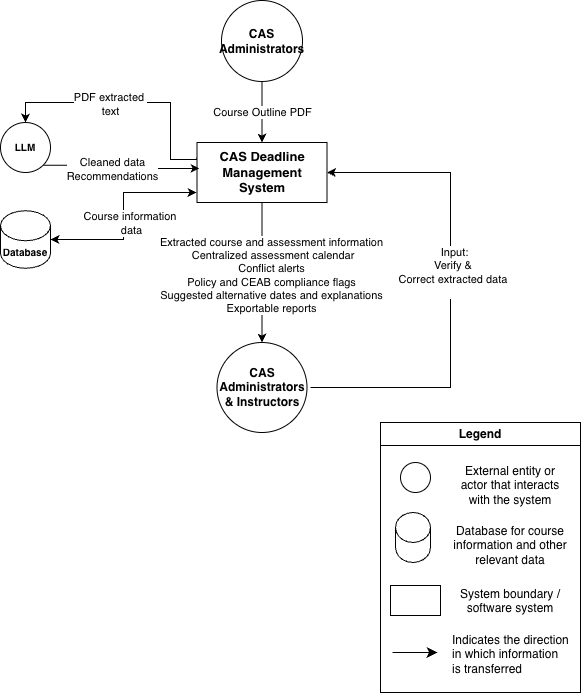
\includegraphics[width=0.6\textwidth]{../SRS-IEEE/SystemContext2.3.png}
\caption{System Context}
\label{Fig_SystemContext} 
\end{center}
\end{figure}

The CAS Deadline Management System is a web-based application intended to support 
course outline review, assessment scheduling, and policy compliance within the CAS Department at 
McMaster University. CAS administrators and course instructors 
interact with the system to upload course outlines, review extracted information, view assessment 
schedules, and evaluate potential scheduling conflicts and compliance issues.
Figure~\ref{Fig_SystemContext} summarizes these interactions by showing the system boundary
and its relationships with instructors, CAS administrators, the LLM, and the database.
\\ \\
The system processes course outlines and relevant academic scheduling information to extract 
assessment details, identify missing or potentially non-compliant information, and recommend 
alternative assessment dates. Results are presented to users for review, while instructors and 
authorized administrators retain responsibility for final scheduling and compliance decisions.
\\ \\
The system is intended for academic administration and planning rather than mission-critical or 
safety-critical applications. Since extracted information and automated recommendations may be 
incomplete or inaccurate, users must review flagged issues and verify important results before 
making decisions.

\begin{itemize}
    \item \textbf{User Responsibilities:}
    \begin{itemize}
        \item Provide course outlines and relevant academic scheduling information.
        \item Ensure submitted documents are appropriate for review and that the information provided is sufficiently complete and accurate.
        \item Review extracted course and assessment information and correct errors where supported.
        \item Evaluate flagged scheduling conflicts, missing information, and potential policy compliance issues.
        \item Decide whether to accept or reject suggested assessment dates and determine any final changes to course schedules.
    \end{itemize}

    \item \textbf{\progname{} Responsibilities:}
    \begin{itemize}
        \item Accept and process supported course outline documents and scheduling information.
        \item Extract and organize relevant course and assessment details for review.
        \item Validate extracted data for missing, inconsistent, or incorrectly formatted values where possible.
        \item Present assessment schedules and identify potential workload conflicts.
        \item Flag potential gaps in course outline requirements and applicable accreditation criteria.
        \item Generate alternative assessment date recommendations with supporting explanations.
        \item Present results and warnings to users without automatically changing course outlines or assessment schedules.
    \end{itemize}

    \item \textbf{External System Responsibilities:}
    \begin{itemize}
        \item \textbf{LLM:} Process course outline content to support information extraction and, where applicable, the generation of explanations for scheduling recommendations.
        \item \textbf{Database:} Store and retrieve course information, extracted assessment details, review results, and scheduling information.
    \end{itemize}
\end{itemize}



\subsection{User Characteristics} \label{SecUserCharacteristics}

The primary users of the CAS Deadline Management System are CAS administrators 
and course instructors at McMaster University. Users are expected to have basic 
computer skills, including navigating web applications and viewing course information. 
CAS administrators should be familiar with course outline reviews, academic scheduling, 
and applicable university policies. Course instructors should have knowledge of their own 
course outlines and assessment schedules. No programming or machine learning knowledge is 
required. Users should be able to review extracted information, interpret flagged issues 
and scheduling recommendations, and make informed decisions regarding their courses or 
administrative responsibilities.

\subsection{System Constraints}

The CAS Deadline Management System must operate within the technical and institutional 
constraints of McMaster University. The following constraints apply to the system:

\begin{itemize}
    \item \textbf{Deployment Environment:} The system must be deployable within 
    the computing resources made available by McMaster University. The availability and 
    capacity of these resources may limit the models and processing workloads the system can support.

    \item \textbf{Data Sources:} The system must process course outlines provided in PDF format. 
    Variations in document structure, formatting, and scan quality may affect the accuracy of 
    information extraction.

    \item \textbf{Language Model Cost and Hosting:} The system must use an LLM that is
    available at no cost to the project. GitHub Copilot should be preferred where it
    satisfies the system's technical and institutional requirements. Otherwise, the
    system should prioritize locally hosted, open-weight language models to minimize
    reliance on external services. Model selection must account for available computing
    resources and applicable licensing restrictions.

    \item \textbf{Human Decision-Making:} The system must not automatically modify course outlines or 
    assessment dates. All scheduling changes and final compliance decisions remain the responsibility 
    of instructors and authorized administrators.

    \item \textbf{Policy and Accreditation Requirements:} Compliance checks must be based on documented 
    McMaster University policies and applicable CEAB requirements. The system must support human review 
    of flagged issues rather than treating automated results as definitive determinations.
\end{itemize}


% ============================================================== 
\section{Stakeholder Requirements}

%\plt{Technology-independent requirements. These come from statements made by
%the stakeholders.  You will find these through interviews and surveys.  They are
%often expressed in natural language. They are not necessarily testable, but
%they should be verifiable.}

%\plt{The stakeholder requirements are numbered so that you can have traceability to other parts of your document.}

\noindent \begin{itemize}
  
\item[SR\refstepcounter{srnum}\thesrnum \label{SR-CAS-01}] Centralized Course Outline Submission: 
CAS administrators need a centralized location to collect and review course outlines.

\item[SR\refstepcounter{srnum}\thesrnum \label{SR-CAS-02}] Course Information Extraction: 
CAS administrators need relevant information extracted from submitted course outlines, including course 
details, assignments and projects, marking schemes, and midterm dates where available.

\item[SR\refstepcounter{srnum}\thesrnum \label{SR-CAS-03}] McMaster Policy Review: 
CAS administrators need support in identifying potential failures of course outlines to comply 
with McMaster University and CAS department policies.

\item[SR\refstepcounter{srnum}\thesrnum \label{SR-CAS-04}] CEAB Accreditation Review: 
CAS administrators need support in reviewing course outlines against CEAB accreditation 
requirements, including evaluating how each course addresses relevant CEAB graduate attributes.

\item[SR\refstepcounter{srnum}\thesrnum \label{SR-REC-01}] Assessment Schedule Analysis: 
Professors/instructors and CAS administrators need to identify periods with high concentrations 
of assessment and midterm deadlines across relevant CAS department courses and reassess 
the schedule when dates are updated.

\item[SR\refstepcounter{srnum}\thesrnum \label{SR-REC-02}] Scheduling Recommendations: 
Professors/instructors need recommendations for alternative midterm and assessment dates 
that may reduce deadline bottlenecks for students, while being able to make the final decision.

\item[SR\refstepcounter{srnum}\thesrnum \label{SR-REC-03}] Instructor Decision-Making:
Professors/instructors need to retain authority over whether to accept or reject scheduling recommendations.

\item[SR\refstepcounter{srnum}\thesrnum \label{SR-REC-04}] Handling Incomplete Information: 
Professors/instructors and CAS administrators need to be informed when missing or unreadable 
course outline information may affect the reliability of compliance reviews or scheduling recommendations.

\item[SR\refstepcounter{srnum}\thesrnum \label{SR-REC-05}] Authorized Access: 
CAS administrators and professors/instructors need access to the information and functions relevant 
to their roles, while assuring sensitive information is protected and restricted to authorized users.

\item[SR\refstepcounter{srnum}\thesrnum \label{SR-REC-06}] Shared Assessment Calendar: 
Professors/instructors and CAS administrators need access to a shared calendar displaying 
relevant course assessment dates.

\item[SR\refstepcounter{srnum}\thesrnum \label{SR-REC-07}] Exam and Restricted-Period Conflicts: 
Professors/instructors and CAS administrators need to identify potential conflicts between 
assessments, exam dates, and applicable restricted periods.

\end{itemize}


%\plt{You should give your SRs meaningful labels, so that you can refer to them
%in other parts of the SRS.  The label names should be meaningful mnemonics, not
%numbers.}

% ============================================================== 
\section{User Personas}
%\plt{Create 2-5 realistic personas.
%  Personas are fictional characters that represent the different user types that
%  might use your software.  They are used to help understand the users'
%  needs, experiences, behaviors and goals.  They are not real people, but they
%  should be based on real data collected from user research.}

\subsection{Persona 1}
\begin{itemize}
\item Name: Bob M. Builder (CAS Administrator)
\item Description: Bob is responsible for collecting and reviewing CAS course outlines 
to help ensure they align with McMaster University and CAS department policies, as well 
as CEAB accreditation requirements. Bob needs an efficient way to carry out his 
administrative duties while reducing the amount of redundant back and forth communication 
with instructors to ensure that outlines are aligned with the required policies and accreditation requirements.

\item Goals: 
\begin{itemize}
  \item To collect and review course outlines in one centralized location.
  \item To identify missing information and potential policy or accreditation issues.
  \item To reduce the time spent manually reviewing multiple course outlines.
  \item To reduce unproductive communication time with course instructors.
\end{itemize}
\item Frustrations:
\begin{itemize}
  \item Course outlines may use different formats or organize information differently.
  \item Manually locating relevant information across many documents can be time-consuming.
  \item Missing or unclear information can make it difficult to assess compliance.
\end{itemize}
\item Technical Ability: Moderate (experience with administrative software, document management tools, spreadsheets)
\end{itemize}


\subsection{Persona 2}
\begin{itemize}
\item Name: Dora Sanchez Explora (Software Engineering Professor)
\item Description: Dora teaches Software Engineering Design courses and plans 
assignments and two midterms for the semester. She wants to provide students with a workload 
that is easy to manage and deadlines that allow them to learn and adequately prepare 
for their midterms without overwhelming them in their other courses.
\item Goals:
\begin{itemize}
  \item To submit and maintain tentative assessment dates efficiently.
  \item To identify potential conflicts with assessments in other courses.
  \item To receive practical recommendations for distributing assessment deadlines more evenly.
  \item To retain final authority over assessment dates for her course.
\end{itemize}
\item Frustrations:
\begin{itemize}
  \item Coordinating assessment dates across courses can be difficult.
  \item Several courses may schedule major assessments around the same time.
  \item Changing an assessment date may create conflicts with other course activities or require additional coordination.
\end{itemize}
\item Technical Ability: Moderate (experience with administrative management systems, online course and university tools)
\end{itemize}


\subsection{Persona 3}
\begin{itemize}
\item Name: Homer Simpson (4th Year Software Engineering Student)
\item Description: Homer is an undergraduate Software Engineering student taking six courses 
for the Fall term. He is feeling overwhelmed by the workload and is struggling to manage his 
time between getting his work done and studying for his upcoming back-to-back midterms. 
\item Goals:
\begin{itemize}
\item To have a more balanced distribution of assessments throughout the term.
\item To avoid periods when multiple major deadlines occur close together.
\item To have sufficient time to prepare for major assessments across different courses.
\end{itemize}
\item Frustrations:
\begin{itemize}
\item Multiple assignments and midterms may fall within the same few days.
\item Heavy assessment periods can make it difficult to allocate study/work time effectively.
\item Assessment dates across different courses may be difficult to coordinate.
\end{itemize}
\item Technical Ability: High (experience with online learning platforms, digital calendars, student productivity tools and software)
\end{itemize}

\subsection{Persona 3}
\begin{itemize}
\item Name:
\item Description:
\item Goals:
\item Frustrations:
\item Technical Ability:
\end{itemize}

% ============================================================== 
\section{Use Cases}
%\plt{Use cases are a way to describe the interactions between users and the system.
%  They are typically written in natural language and describe the steps that a
%  user takes to achieve a specific goal.  Use cases can be used to identify
%  functional requirements and to create test cases.}  
%\plt{Typically 8-15 substantial use cases.}

\refstepcounter{ucnum} \label{UC_CAS_01}
\subsection{\ucref{UC_CAS_01}: Submit Course Outline}

\noindent \textbf{Primary Actor:} CAS Administrator

\noindent \textbf{Preconditions}
\begin{itemize}
  \item The administrator has access to the system.
  \item A CAS course outline is available for submission.
\end{itemize}

\noindent \textbf{Main Success Scenario}
\begin{enumerate}
  \item The administrator logs into the system.
  \item The administrator selects the option to submit a course outline.
  \item The administrator selects and submits the course outline.
  \item The system receives the document and attempts to extract relevant course information.
  \item The system confirms that the course outline has been submitted successfully.
  \item The system makes the submitted outline available for information extraction and review.
\end{enumerate}

\noindent \textbf{Alternative Flows}
\begin{itemize}
  \item If the submitted document cannot be read, the system informs the administrator that a readable document is required.
  \item If the submission fails, the system informs the administrator and allows them to try again.
  \item If relevant course information is missing, the system proceeds with the information that is available and identifies the missing information.
  \item If the Copilot or LLM service is unavailable, the system informs the administrator that automatic information extraction cannot be completed. The submitted course outline remains available, and the administrator can retry extraction when the service becomes available.
\end{itemize}

\noindent \textbf{Postconditions}
\begin{itemize}
  \item If submission succeeds, the course outline is stored and available for review, even if automatic information extraction could not be completed.
  \item If submission fails, the administrator is informed that the course outline was not submitted successfully.
\end{itemize}



\refstepcounter{ucnum} \label{UC_CAS_02}
\subsection{\ucref{UC_CAS_02}: Review Extracted Course Information}

\noindent \textbf{Primary Actor:} CAS Administrator

\noindent \textbf{Preconditions}
\begin{itemize}
  \item A course outline has been submitted successfully.
  \item The system has attempted to extract relevant course information.
\end{itemize}

\noindent \textbf{Main Success Scenario}
\begin{enumerate}
  \item The administrator selects a submitted course outline.
  \item The system presents the extracted course details and information, including assignments, marking schemes, and midterm dates where available, and flags any missing, uncertain, or ambiguous information for review.
  \item The administrator reviews the extracted information against the original course outline.
  \item The administrator fills in any missing information or confirms that the information is correct.
  \item The system saves the verified course information for later steps and scheduling analysis.
\end{enumerate}

\noindent \textbf{Alternative Flows}
\begin{itemize}
  \item If the system cannot extract certain information, it identifies the missing information for the administrator to review.
  \item If the system extracts information that is uncertain or ambiguous, it flags the affected information for administrator review and indicates that verification is required.
  \item If the administrator identifies incorrect information, they correct it before proceeding.
\end{itemize}

\noindent \textbf{Postconditions}
\begin{itemize}
  \item The extracted course information has been reviewed and corrected where necessary.
\end{itemize}



\refstepcounter{ucnum} \label{UC_CAS_03}
\subsection{\ucref{UC_CAS_03}: Review Course Outline Against McMaster and CAS Policies}

\noindent \textbf{Primary Actor:} CAS Administrator

\noindent \textbf{Preconditions}
\begin{itemize}
  \item A course outline has been submitted.
  \item Relevant course information is available for review.
  \item McMaster University and CAS department policy criteria are available to the system.
\end{itemize}

\noindent \textbf{Main Success Scenario}
\begin{enumerate}
  \item The administrator selects a course outline for policy review.
  \item The system evaluates the available course information against policy criteria.
  \item The system identifies potential policy inconsistencies or missing required information.
  \item The system presents the findings and supporting information to the administrator.
  \item The administrator reviews the findings and determines which issues require further investigation or correction.
\end{enumerate}

\noindent \textbf{Alternative Flows}
\begin{itemize}
  \item If relevant information is missing, the system identifies the limitation and presents any findings that can still be supported.
  \item If a potential policy issue cannot be determined conclusively, the system flags it for manual review.
  \item If the necessary policy criteria are unavailable, the system informs the administrator that the review cannot be completed reliably.
\end{itemize}

\noindent \textbf{Postconditions}
\begin{itemize}
  \item The administrator has access to policy review findings and can identify issues requiring further attention.
\end{itemize}


\refstepcounter{ucnum} \label{UC_CAS_04}
\subsection{\ucref{UC_CAS_04}: Review Course Outline Against CEAB Criteria}

\noindent \textbf{Primary Actor:} CAS Administrator

\noindent \textbf{Preconditions}
\begin{itemize}
  \item A course outline has been submitted.
  \item Relevant course information is available for review.
  \item Applicable CEAB accreditation criteria are available to the system.
\end{itemize}

\noindent \textbf{Main Success Scenario}
\begin{enumerate}
  \item The administrator selects a course outline for CEAB-related review.
  \item The system evaluates the available course information against CEAB criteria.
  \item The system identifies potential information gaps that may require further examination.
  \item The system presents the findings and supporting information to the administrator.
  \item The administrator reviews the findings and determines which issues require further investigation or correction.
\end{enumerate}

\noindent \textbf{Alternative Flows}
\begin{itemize}
  \item If relevant information is missing, the system identifies the limitation and presents any findings that can still be supported.
  \item If a potential gap requires professional judgment, the system flags it for manual review.
  \item If the necessary CEAB criteria are unavailable, the system informs the administrator that the review cannot be completed reliably.
\end{itemize}

\noindent \textbf{Postconditions}
\begin{itemize}
  \item The administrator has access to CEAB-related review findings and can identify issues requiring further attention.
\end{itemize}



\refstepcounter{ucnum} \label{UC_CAS_05}
\subsection{\ucref{UC_CAS_05}: Review Course Outline Findings}

\noindent \textbf{Primary Actor:} CAS Administrator

\noindent \textbf{Preconditions}
\begin{itemize}
  \item A course outline has been submitted.
  \item At least one policy or CEAB-related review has been performed.
\end{itemize}

\noindent \textbf{Main Success Scenario}
\begin{enumerate}
  \item The administrator opens the review findings for a course outline.
  \item The system displays identified potential issues, missing information, and relevant supporting details.
  \item The administrator examines the findings and determines required follow-up.
  \item The administrator uses the findings to support the course outline review process.
\end{enumerate}

\noindent \textbf{Alternative Flows}
\begin{itemize}
  \item If no potential issues are identified, the system indicates that no issues were detected by the review.
  \item If the findings depend on incomplete or uncertain information, the system identifies those limitations.
\end{itemize}

\noindent \textbf{Postconditions}
\begin{itemize}
  \item The administrator has reviewed the available findings and identified any issues requiring follow-up.
\end{itemize}


\refstepcounter{ucnum} \label{UC_PROF_01}
\subsection{\ucref{UC_PROF_01}: Submit Tentative Assessment Dates}

\noindent \textbf{Primary Actor:} Professor/Instructor

\noindent \textbf{Preconditions}
\begin{itemize}
  \item The professor or instructor has access to the system.
  \item The instructor has tentative assessment dates for a relevant course.
\end{itemize}

\noindent \textbf{Main Success Scenario}
\begin{enumerate}
  \item The instructor selects the relevant course.
  \item The instructor enters or submits tentative dates for assessments and midterms.
  \item The system checks the submitted information for completeness.
  \item The system presents any identified missing or invalid information to the instructor.
  \item The instructor corrects any identified issues and submits the information.
  \item The system saves the tentative assessment dates for scheduling analysis.
\end{enumerate}

\noindent \textbf{Alternative Flows}
\begin{itemize}
  \item If required assessment information is missing, the system identifies the missing details and asks the instructor to complete them.
  \item If a date is invalid or cannot be interpreted, the system asks the instructor to correct it.
  \item If the instructor needs to revise the submitted dates, they can update the information and submit it again.
\end{itemize}

\noindent \textbf{Postconditions}
\begin{itemize}
  \item The instructor's tentative assessment dates are stored and available for scheduling analysis.
\end{itemize}


\refstepcounter{ucnum} \label{UC_PROF_02}
\subsection{\ucref{UC_PROF_02}: Analyze Assessment Schedule}

\noindent \textbf{Primary Actor:} Professor/Instructor, CAS Administrator

\noindent \textbf{Preconditions}
\begin{itemize}
  \item The user has access to the system.
  \item Assessment dates are available for the relevant courses, if any have been submitted.
\end{itemize}

\noindent \textbf{Main Success Scenario}
\begin{enumerate}
  \item The instructor requests an analysis of the assessment schedule.
  \item The system gathers the available assessment dates for relevant courses.
  \item The system analyzes the distribution of assessments and midterms across the relevant period.
  \item The system identifies periods with high concentrations of assessments or potential student workload bottlenecks.
  \item The system presents the analysis results to the instructor.
\end{enumerate}

\noindent \textbf{Alternative Flows}
\begin{itemize}
  \item If assessment information is incomplete, the system identifies the missing information and explains how it limits the analysis.
  \item If insufficient assessment dates are available, the system informs the instructor that a reliable analysis cannot be completed.
  \item If no significant bottlenecks are identified, the system presents the analysis without recommending unnecessary changes.
  \item If the instructor or administrator wants to view the assessment calendar without performing an analysis, they can filter the calendar by academic year and program. The system displays the assessment dates matching the selected filters without generating workload analysis or recommendations.
\end{itemize}

\noindent \textbf{Postconditions}
\begin{itemize}
  \item The instructor or administrator can review the assessment schedule, either through the calendar view or through the results of a schedule analysis, depending on the requested operation.
\end{itemize}


\refstepcounter{ucnum} \label{UC_PROF_03}
\subsection{\ucref{UC_PROF_03}: Generate Scheduling Recommendations}

\noindent \textbf{Primary Actor:} Professor/Instructor

\noindent \textbf{Preconditions}
\begin{itemize}
  \item An assessment schedule analysis has been completed.
  \item Sufficient information is available to identify potential alternative dates.
\end{itemize}

\noindent \textbf{Main Success Scenario}
\begin{enumerate}
  \item The instructor requests scheduling recommendations based on the available assessment schedule.
  \item The system identifies assessments that contribute to periods with high concentrations of deadlines.
  \item The system evaluates potential alternative dates for affected assessments.
  \item The system generates recommendations intended to reduce assessment bottlenecks while considering the available scheduling information.
  \item The system presents the suggested dates and the available reasoning behind the recommendations.
  \item The instructor reviews the recommendations.
\end{enumerate}

\noindent \textbf{Alternative Flows}
\begin{itemize}
  \item If no suitable alternative dates can be identified, the system informs the instructor that it cannot provide a suitable recommendation.
  \item If relevant scheduling information is missing, the system identifies the limitation.
  \item If several alternatives are available, the system presents the alternatives for the instructor to evaluate.
  \item If the LLM/Copilot service goes down, the system notifies the instructor, prevents showing false explanations, and allows retrying once the service recovers.
\end{itemize}

\noindent \textbf{Postconditions}
\begin{itemize}
  \item Scheduling recommendations (if applicable) are presented to the instructor for consideration. No assessment dates are changed automatically.
\end{itemize}


\refstepcounter{ucnum} \label{UC_PROF_04}
\subsection{\ucref{UC_PROF_04}: Review and Decide on Scheduling Recommendations}

\noindent \textbf{Primary Actor:} Professor/Instructor

\noindent \textbf{Preconditions}
\begin{itemize}
  \item Scheduling recommendations have been generated for the relevant assessment schedule.
\end{itemize}

\noindent \textbf{Main Success Scenario}
\begin{enumerate}
  \item The instructor opens the scheduling recommendations.
  \item The system displays the suggested assessment dates and the rationale for each recommendation.
  \item The instructor evaluates the suggestions against course-specific constraints and other relevant considerations.
  \item The instructor chooses to accept, reject, or modify a proposed date.
  \item The system records the instructor's decision and updates the schedule if an accepted or modified date is submitted.
\end{enumerate}

\noindent \textbf{Alternative Flows}
\begin{itemize}
  \item If the instructor rejects a recommendation, the existing assessment date remains unchanged.
  \item If the instructor modifies a recommendation, the system allows the revised date to be submitted.
  \item If the instructor needs more information, they can review the schedule analysis before making a decision.
\end{itemize}

\noindent \textbf{Postconditions}
\begin{itemize}
  \item The instructor's decision is reflected in the schedule where an update has been submitted. Rejected recommendations do not change the existing assessment dates.
\end{itemize}



\refstepcounter{ucnum} \label{UC_PROF_05}
\subsection{\ucref{UC_PROF_05}: Update Assessment Dates and Re-analyze Schedule}

\noindent \textbf{Primary Actor:} Professor/Instructor

\noindent \textbf{Preconditions}
\begin{itemize}
  \item Assessment dates for the relevant course have previously been submitted.
  \item The instructor has identified a need to change one or more tentative assessment dates.
\end{itemize}

\noindent \textbf{Main Success Scenario}
\begin{enumerate}
  \item The instructor selects the relevant course and assessment schedule.
  \item The instructor updates one or more tentative assessment dates.
  \item The system checks the updated information for completeness and validity, then saves the updated dates.
  \item The instructor requests a new assessment schedule analysis.
  \item The system analyzes the updated schedule and identifies any remaining or newly introduced bottlenecks.
  \item The system presents the updated analysis and any resulting recommendations.
\end{enumerate}

\noindent \textbf{Alternative Flows}
\begin{itemize}
  \item If an updated date is invalid or incomplete, the system asks the instructor to correct it before proceeding.
  \item If insufficient information is available for re-analysis, the system identifies the missing information.
  \item If the updated schedule introduces new bottlenecks, the system identifies them in the new analysis.
\end{itemize}

\noindent \textbf{Postconditions}
\begin{itemize}
  \item The updated tentative assessment dates are available in the system, and a new analysis is available if sufficient information was provided.
\end{itemize}

% ============================================================== 
\section{Functional Requirements}

\noindent The system shall support the following capabilities, grouped by feature area.

\subsection*{Outline Intake and Extraction}
\begin{itemize}
\item[FR\refstepcounter{reqnum}\thereqnum \label{FR_Intake_Data}:] The system shall accept course outlines in PDF format submitted by a CAS administrator or professor.
\item[FR\refstepcounter{reqnum}\thereqnum \label{FR_Extract_Assessment}:] The system shall extract each assessment's name, type, date, and weight from a course outline.
\item[FR\refstepcounter{reqnum}\thereqnum \label{FR_Extract_LO}:] The system shall extract the learning outcomes and graduate attribute numbers listed in a course outline.
\item[FR\refstepcounter{reqnum}\thereqnum \label{FR_Extract_Flag}:] The system shall flag any extracted field that is missing, including a date that is marked TBD.
\item[FR\refstepcounter{reqnum}\thereqnum \label{FR_Extract_Review}:] The system shall require a user to review and confirm extracted data before it is used for the calendar, conflict detection, or compliance checking.
\item[FR\refstepcounter{reqnum}\thereqnum \label{FR_Dates_Tentative}:] The system shall allow an instructor to enter and update tentative assessment dates for their own courses.
\end{itemize}

\subsection*{Calendar and Conflict Detection}
\begin{itemize}
\item[FR\refstepcounter{reqnum}\thereqnum \label{FR_Calendar}:] The system shall display confirmed and tentative assessment dates in a shared calendar that can be filtered by course, year, and program, with tentative dates marked as such.
\item[FR\refstepcounter{reqnum}\thereqnum \label{FR_Work_Cluster}:] The system shall identify weeks in which a student cohort has more assessments than a configurable threshold.
\item[FR\refstepcounter{reqnum}\thereqnum \label{FR_Work_Policy}:] The system shall identify assessments scheduled in periods restricted by McMaster policy, such as final exam periods.
\item[FR\refstepcounter{reqnum}\thereqnum \label{FR_Reanalyze}:] The system shall re-run conflict detection for the affected courses and cohorts whenever an assessment date is added or changed.
\end{itemize}

\subsection*{Scheduling Suggestions}
\begin{itemize}
\item[FR\refstepcounter{reqnum}\thereqnum \label{FR_Suggest_Generation}:] The system shall, on explicit request by the instructor, suggest alternative dates, for assessments involved in a detected conflict or listed as TBD.
\item[FR\refstepcounter{reqnum}\thereqnum \label{FR_Suggest_NoAuto}:] The system shall not change any assessment date without the explicit approval of the responsible instructor.
\end{itemize}

\subsection*{Compliance Checking}
\begin{itemize}
\item[FR\refstepcounter{reqnum}\thereqnum \label{FR_Comp_Policy}:] The system shall check each outline against the McMaster course outline policy rules, including required sections and assessment weights totalling 100\%, and report each finding.
\item[FR\refstepcounter{reqnum}\thereqnum \label{FR_Comp_Grad}:] The system shall compare the graduate attribute numbers in an outline with the master course sheet and flag any that are missing or inconsistent.
\end{itemize}

\subsection*{Access and Export}
\begin{itemize}
\item[FR\refstepcounter{reqnum}\thereqnum \label{FR_Access_Login}:] The system shall require users to log in before they can view or change any data.
\item[FR\refstepcounter{reqnum}\thereqnum \label{FR_Access_Roles}:] The system shall allow administrators to manage data for all courses, and shall allow instructors to change data only for their own courses.
\item[FR\refstepcounter{reqnum}\thereqnum \label{FR_Export_CSV}:] The system shall allow an administrator to export extracted assessment data as a CSV file.
\end{itemize}

% \subsection*{Notifications}
% \begin{itemize}
% \item[FR\refstepcounter{reqnum}\thereqnum \label{FR_Notify_Email}:] The system shall send scheduling suggestions and compliance results to instructors by email, and display on the website.
% \end{itemize}

% ============================================================== 
\section{Data Requirements}

\subsection{Major Data Entities}

\begin{itemize}
\item \textbf{User:} an administrator or instructor. Both can submit outlines and confirm extracted data. Instructors also enter tentative dates, and request and approve date suggestions, for their own courses.
\item \textbf{Course:} a CAS course offering in a given term, taught by one instructor. A course may be cross-listed. SFWRENG 4X03, COMPSCI 3X03, and MECHTRON 3X03 are one course taught by one instructor, with a separate course code for each program. The outline and its assessments are stored once.
\item \textbf{CourseCode:} one listing of a course. Each code belongs to one course, and a course has one or more codes. The program and year level are derived from the code and are not entered separately.
\item \textbf{CourseOutline:} a submitted course outline PDF. Each outline belongs to one course, including when that course has several course codes.
\item \textbf{Assessment:} a graded component of a course (midterm, assignment, lab, etc.) with a weight and a date. The date is empty when it is missing or TBD, and an instructor can enter a tentative date.
\item \textbf{LearningOutcome:} a learning outcome stated in an outline, with any graduate attribute numbers listed beside it. A user reviews each outcome after extraction, and the review status records whether it is still extracted or has been confirmed.
\item \textbf{MasterCourseRecord:} a row of the master course sheet, listing the graduate attribute numbers expected for a course code. A cross-listed course can match more than one row, one for each of its codes.
\item \textbf{AcademicCalendarEntry:} a holiday, exam period, or other restricted date range.
\item \textbf{DateRecommendation:} a suggested alternative date for an assessment, with its explanation and decision.
\item \textbf{ComplianceFinding:} a problem found when checking an outline against McMaster policy or the master course sheet.
\end{itemize}

\noindent An instructor teaches one or more courses. Each course has one or more course codes and one or more outlines. Each outline contains many assessments and learning outcomes, stored once for the course rather than once per course code. Student cohorts are found by grouping course codes that share the same derived program and year level. Workload conflicts are calculated from the stored assessments when needed, so neither cohorts nor conflicts are stored separately.

\subsection{Data Dictionary}

{\footnotesize
\setlength{\LTleft}{0pt}
\setlength{\LTright}{0pt}
\renewcommand{\arraystretch}{1.2}

\begin{longtable}{|>{\raggedright\arraybackslash}p{0.23\linewidth}|>{\raggedright\arraybackslash}p{0.67\linewidth}|}
\caption{Data Dictionary}\label{tab:data-dictionary}\\
\hline
\textbf{Entity} & \textbf{Attributes (type): description} \\ \hline
\endfirsthead

\hline
\textbf{Entity} & \textbf{Attributes (type): description} \\ \hline
\endhead

User &
user\_id (UUID): unique identifier. \newline
email (String): user's email address. \newline
role (Enum): administrator or instructor. \\ \hline

Course &
course\_id (UUID): unique identifier. \newline
instructor\_id (UUID): user who teaches the course. \newline
term (String): academic term of the offering. \\ \hline

CourseCode &
course\_code\_id (UUID): unique identifier. \newline
course\_id (UUID): course this listing belongs to. \newline
code (String): course code, e.g., SFWRENG 4X03. \newline
program (String, derived): program inferred from the subject in the code, for example Software Engineering from SFWRENG. Not entered separately. \newline
year\_level (Integer, derived): program year inferred from the first digit of the course number, for example 4 in SFWRENG 4X03 and 3 in COMPSCI 3X03. Not entered separately. \\ \hline

CourseOutline &
outline\_id (UUID): unique identifier. \newline
course\_id (UUID): course the outline belongs to. \newline
submitted\_at (Timestamp): when the outline was submitted. \\ \hline

Assessment &
assessment\_id (UUID): unique identifier. \newline
outline\_id (UUID): outline the assessment was extracted from. \newline
name (String): name as written in the outline. \newline
type (Enum): midterm, assignment, quiz, lab, project, final exam, other. \newline
due\_date (Date or null): null when missing or TBD. \newline
is\_tentative (Boolean): true when the date was entered by an instructor and is not final. \newline
weight\_percent (Decimal): percentage of the final grade. \newline
review\_status (Enum): extracted or confirmed. \newline
source\_text (String): outline text the values were extracted from. \\ \hline

LearningOutcome &
outcome\_id (UUID): unique identifier. \newline
outline\_id (UUID): outline the outcome appears in. \newline
text (String): outcome as written. \newline
ga\_numbers (List of Integer): graduate attribute numbers listed in the outline. \newline
review\_status (Enum): extracted or confirmed. \newline
source\_text (String): outline text the values were extracted from. \\ \hline

MasterCourseRecord &
course\_code (String): course code this row applies to. Matches a CourseCode. \newline
expected\_ga\_numbers (List of Integer): attribute numbers the master sheet lists for that course code. \\ \hline

AcademicCalendarEntry &
start\_date (Date): start of the range. \newline
end\_date (Date): end of the range. \newline
restriction (Enum): holiday, exam period, no-assessment period. \\ \hline

DateRecommendation &
recommendation\_id (UUID): unique identifier. \newline
assessment\_id (UUID): assessment the suggestion applies to. \newline
suggested\_date (Date): proposed date. \newline
explanation (String): reason for the suggestion, shown to the instructor. \newline
decision (Enum): pending, accepted, rejected. \\ \hline

ComplianceFinding &
finding\_id (UUID): unique identifier. \newline
outline\_id (UUID): outline that was checked. \newline
message (String): description of the problem found. \\ \hline
\end{longtable}
}

\subsection{Privacy and Data Retention} \label{SecPrivacyDataRetention}

\begin{itemize}

\item[DR\refstepcounter{drnum}\thedrnum \label{DR_Confidentiality}:] Course outlines and the data extracted from them are generally public. The master course sheet and other department data may be confidential, and shall only be available to authorized CAS users.

\item[DR\refstepcounter{drnum}\thedrnum \label{DR_Hosting}:] Course and department data shall be processed on CAS-hosted infrastructure. GitHub Copilot is an external service and may be used during development. Only publicly available course outline information may be sent to Copilot. Confidential department data and student personal information shall not be sent to Copilot or to any other external service.

\item[DR\refstepcounter{drnum}\thedrnum \label{DR_Access}:] Users shall only see and change the data their role allows.

\item[DR\refstepcounter{drnum}\thedrnum \label{DR_Retention}:] The retention period for outlines, extracted data, and findings shall be 10 years. The Undergraduate Course Management Policy requires that course outlines be retained for at least 10 years.

\end{itemize}

% ============================================================== 
\section{Non-Functional Requirements}

\noindent \begin{itemize}

\item[NFR\refstepcounter{nfrnum}\thenfrnum \label{NFR_Accuracy}:]
\textbf{Accuracy:}
\begin{itemize}
    \item The system shall achieve at least 95\% accuracy for extracted assessment dates and
    weights on a representative test dataset of course outlines.
    \item The system shall achieve at least 95\% recall for predefined missing or incomplete
    information in the same test dataset.
    \item The system shall identify at least 95\% of predefined policy and CEAB compliance
    issues and report the results in the Verification and Validation Plan.
    \item These thresholds align with the success measures in the Problem Statement and
    Goals document.
\end{itemize}

\item[NFR\refstepcounter{nfrnum}\thenfrnum \label{NFR_Usability}:]
\textbf{Usability:}
\begin{itemize}
    \item The system shall allow the CAS administrators and course instructors described in
    Section~\ref{SecUserCharacteristics} to upload course outlines, review extracted information,
    view assessment schedules, and interpret flagged issues without programming or machine
    learning knowledge.
    \item At least 80\% of participants in representative usability testing shall complete
    each designated core task without assistance.
    \item The 80\% target is a project-defined validation threshold intended to demonstrate
    that the core workflows are usable by the intended non-technical users.
\end{itemize}

\item[NFR\refstepcounter{nfrnum}\thenfrnum \label{NFR_Maintainability}:]
\textbf{Maintainability:}
\begin{itemize}
    \item The system shall be organized into modular components for document processing,
    information extraction, scheduling analysis, and compliance rules.
    \item Changes to one of these components shall not require unrelated components to be
    rewritten.
    \item For representative maintenance tasks defined in the Verification and Validation
    Plan, the effort required to implement each change shall be documented and assessed
    against the original implementation effort for the affected component.
\end{itemize}

\item[NFR\refstepcounter{nfrnum}\thenfrnum \label{NFR_Portability}:]
\textbf{Portability:}
\begin{itemize}
    \item The system shall be deployable in the designated McMaster University hosting
    environment.
    \item The system shall be usable through Google Chrome 120 or later, Mozilla Firefox 121
    or later, and Safari 17 or later on supported desktop operating systems.
    \item The deployment and core workflow tests defined in the Verification and Validation
    Plan shall be executed in each supported browser environment. These browser versions
    define the project's verification baseline and may be updated for a future release.
\end{itemize}

\item[NFR\refstepcounter{nfrnum}\thenfrnum \label{NFR_Installability}:]
\textbf{Installability and Deployability:}
\begin{itemize}
    \item A new maintainer shall be able to deploy the system to the designated McMaster
    University hosting environment by following the documented installation and deployment
    instructions.
    \item The documented procedure shall identify required software, configuration values,
    environment variables, database setup, and service startup steps without relying on
    undocumented knowledge.
    \item The deployment shall be verified by a deployment test in the Verification and
    Validation Plan, including confirmation that the deployed system supports the core
    workflows.
\end{itemize}

\item[NFR\refstepcounter{nfrnum}\thenfrnum \label{NFR_Performance}:]
\textbf{Performance:}
\begin{itemize}
    \item Under the test environment and workload defined in the Verification and Validation
    Plan, the system shall display previously processed assessment calendar data within 3
    seconds for at least 95\% of requests.
    \item For a supported course outline of up to 30 pages, the system shall complete document
    processing and information extraction within 60 seconds for at least 90\% of test runs,
    excluding failures or delays caused by unavailable external dependencies.
    \item The test environment, document characteristics, workload, and response-time results
    shall be recorded.
    \item The 3-second target is a project-defined interactive response target, while the
    60-second target bounds processing time for a typical supported outline; both targets
    shall be validated under the controlled conditions defined in the Verification and
    Validation Plan.
\end{itemize}

\item[NFR\refstepcounter{nfrnum}\thenfrnum \label{NFR_Reliability}:]
\textbf{Reliability:}
\begin{itemize}
    \item The system shall handle invalid, incomplete, or unsupported input documents without
    crashing or corrupting previously stored information.
    \item All predefined invalid-input cases shall produce an appropriate error message, and
    previously stored records shall remain accessible after a failed upload or processing
    attempt.
    \item If the LLM or Copilot service is unavailable, the system shall continue to support
    viewing and editing stored course and assessment information, viewing the assessment
    calendar, and exporting available data.
    \item Submitted course outlines shall be retained, and users shall be able to retry
    extraction or recommendations when the service becomes available, as described in
    \ucref{UC_CAS_01} and \ucref{UC_PROF_03}.
\end{itemize}

\item[NFR\refstepcounter{nfrnum}\thenfrnum \label{NFR_Security}:]
\textbf{Security:}
\begin{itemize}
    \item The system shall implement the access controls specified in \rref{FR_Access_Login}
    and \rref{FR_Access_Roles}, together with the privacy and data-retention requirements
    in Section~\ref{SecPrivacyDataRetention}.
    \item Security verification shall include tests for unauthorized access, role-based
    permissions, and the protection of sensitive configuration values and credentials.
\end{itemize}

\item[NFR\refstepcounter{nfrnum}\thenfrnum \label{NFR_Accessibility}:]
\textbf{Accessibility:}
\begin{itemize}
    \item The system's web interface shall conform to the applicable requirements of the
    \href{https://www.ontario.ca/laws/regulation/110191}{Accessibility for Ontarians with
    Disabilities Act (AODA)} and
    \href{https://www.w3.org/TR/WCAG20/}{WCAG 2.0 Level AA}.
    \item Core workflows, including authentication, course-outline submission, information
    review, calendar viewing, and data export, shall be operable using keyboard navigation
    and shall provide accessible labels, headings, focus indicators, and error messages.
    \item Accessibility verification shall include an automated accessibility scan and
    manual keyboard and screen-reader checks for the core workflows. The applicable WCAG
    success criteria and test results shall be recorded in the Verification and Validation
    Plan.
\end{itemize}

\end{itemize}



% ============================================================== 
\section{AI and Machine Learning Requirements}

\noindent The system extracts information from course outline PDFs in two steps. First, a Python PDF text extraction library reads the text from each PDF. Then a large language model (LLM) cleans up that text and organizes it into structured data. The LLM also compares the graduate attribute numbers in an outline with the master course sheet. The date suggestions come from a constraint solver (CP-SAT), and the assessment weight check is ordinary deterministic code, so neither uses the LLM. In operation the LLM is hosted on CAS infrastructure and kept behind a replaceable interface, so the model can be changed without changing the rest of the system. During development, GitHub Copilot may be used in its place. Copilot is an external service, and the only model input that may be sent to it is publicly available course outline text (\drref{DR_Hosting}).

\subsection{Model Inputs}

\begin{itemize}
\item[AIR\refstepcounter{airnum}\theairnum \label{AIR_Input_Text}:] The model shall receive the text that the PDF extraction library produced from each course outline, rather than the PDF file itself, together with the contents of the master course Excel sheet.
\item[AIR\refstepcounter{airnum}\theairnum \label{AIR_Input_Privacy}:] The operational model shall be hosted on CAS-operated infrastructure. When GitHub Copilot is used during development, only publicly available course outline text may be sent to it (\drref{DR_Hosting}). No student personal information shall be used as model input.
\end{itemize}

\subsection{Model Outputs}

\begin{itemize}
\item[AIR\refstepcounter{airnum}\theairnum \label{AIR_Output_Struct}:] The model shall organize the extracted outline text into structured data containing, for each assessment, its name, type, date, and weight, and for each learning outcome, its text and the graduate attribute numbers listed beside it (\rref{FR_Extract_Assessment}, \rref{FR_Extract_LO}).
\item[AIR\refstepcounter{airnum}\theairnum \label{AIR_Output_Source}:] Every structured value shall include the passage of extracted text it was taken from, so a reviewer can check it without opening the original document.
\item[AIR\refstepcounter{airnum}\theairnum \label{AIR_Output_Missing}:] The model shall only use information present in the extracted text, and shall report a value as missing, including a date that is marked TBD or is too vague to resolve, instead of inventing one (\rref{FR_Extract_Flag}).
\item[AIR\refstepcounter{airnum}\theairnum \label{AIR_Output_Review}:] No model output shall be used for the calendar, conflict detection, or compliance results until a user has confirmed it (\rref{FR_Extract_Review}).
\end{itemize}

\subsection{Evaluation Metrics}

\noindent Each metric shall be measured on a set of sample course outlines, using an answer key prepared manually by the team as the reference. Extraction metrics are measured on the final structured output, so they cover the PDF library and the model together.

{\footnotesize
\setlength{\LTleft}{0pt}
\setlength{\LTright}{0pt}
\renewcommand{\arraystretch}{1.2}

\begin{longtable}{|>{\raggedright\arraybackslash}p{0.22\linewidth}|>{\raggedright\arraybackslash}p{0.38\linewidth}|>{\raggedright\arraybackslash}p{0.20\linewidth}|}
\caption{Evaluation Metrics}\label{tab:ai-metrics}\\
\hline
\textbf{Metric} & \textbf{What it measures} & \textbf{Target} \\ \hline
\endfirsthead

\hline
\textbf{Metric} & \textbf{What it measures} & \textbf{Target} \\ \hline
\endhead

Extraction accuracy & Share of assessment dates and weights that are correct in the final structured output (\rref{FR_Extract_Assessment}) & At least 90\% \\ \hline
Missing-field detection & Share of missing or TBD fields that are flagged (\rref{FR_Extract_Flag}) & At least 90\% \\ \hline
Compliance issue detection & Share of known compliance issues that are found (\rref{FR_Comp_Policy}, \rref{FR_Comp_Grad}) & At least 90\% \\ \hline
\end{longtable}
}

\subsection{Known Limitations}

\noindent The table lists the expected failure modes and how the design contains each one. The main safeguard is that a person confirms every extracted value, with the source text shown beside it. During evaluation, the team also manually reviews a sample of the outputs.

{\footnotesize
\setlength{\LTleft}{0pt}
\setlength{\LTright}{0pt}
\renewcommand{\arraystretch}{1.2}

\begin{longtable}{|>{\raggedright\arraybackslash}p{0.22\linewidth}|>{\raggedright\arraybackslash}p{0.28\linewidth}|>{\raggedright\arraybackslash}p{0.32\linewidth}|}
\caption{Expected Failure Modes}\label{tab:ai-limitations}\\
\hline
\textbf{Failure mode} & \textbf{Effect} & \textbf{Mitigation} \\ \hline
\endfirsthead

\hline
\textbf{Failure mode} & \textbf{Effect} & \textbf{Mitigation} \\ \hline
\endhead

PDF library returns messed up or incomplete text (tables, multiple columns, scanned pages) & Dates, weights, or sections are missing or out of order before the model sees them & Flag outlines with little or no extracted text for manual entry; test on outlines with a range of layouts \\ \hline
Model changes or adds values while cleaning up the text & A date or weight that differs from, or appears nowhere in, the outline & Show the source text; reject values with no source passage; require review \\ \hline
Ambiguous dates, such as ``week of Oct 20'' or ``TBD'' & A date cannot be resolved without a person & Report the date as missing and never guess \\ \hline
Reviewer over-trusts the output & Wrong values are confirmed without being checked & Show the source beside each value; confirm explicitly, never by default \\ \hline
Courses missing from the master sheet (technical electives, mechatronics, computer science) & Attribute comparison is not possible & Tell the user the course was not checked, rather than showing no findings \\ \hline
Uneven accuracy across layouts or programs & Some instructors see more errors than others & Test on outlines from each program; add examples from weak areas \\ \hline
CEAB requirements are not exhaustive & A clean result does not mean full accreditation compliance & State that only the encoded rules were checked \\ \hline
LLM unavailable & Extraction and scheduling explanations cannot be completed & Inform the user, keep the submitted outline, do not present an explanation that was not generated, and allow a retry when the service returns (UC\_CAS\_01, UC\_PROF\_03) \\ \hline
\end{longtable}
}

% ============================================================== 
\section{Requirements Traceability Matrices}

\plt{The Requirements Traceability Matrix (RTM) is a table that shows the
relationship between different types of requirements. It is used to ensure that
all requirements are traceable and that no requirements are missed. The typical
flow is: Stakeholder Need -> Use Case -> Requirement}

\plt{There is also a traceability matrix between functional and nonfunctional
  requirements. The purpose of some FRs is to satisfy NFRs.  Therefore, it is
  important to show the relationship between the two.}

\plt{Further traceability to test cases and modules will be given in other
documents.}

\begin{longtable}{p{0.15\textwidth} p{0.15\textwidth} p{0.20\textwidth} p{0.20\textwidth}}

\toprule
Stakeholder Req & Use Case & Functional Req \\
\midrule
\srref{SR_Label1} & \ucref{UC_Label1} & \rref{FR_Label1} \\
\bottomrule

\caption{Traceability Between Stakeholder Requirements, Use Cases, and
Functional Requirements} \label{tab:SR2UC2FRtm}
\end{longtable}

\begin{longtable}{p{0.20\textwidth} p{0.20\textwidth}}

\toprule
Functional Req & Nonfunctional Req \\
\midrule
\rref{FR_Label1} & \nfrref{NFR_Accuracy} \\
\bottomrule
\caption{Traceability Between Functional and Nonfunctional Requirements}
\label{tab:FR2Rtm}

\end{longtable}

\begin{longtable}{p{0.28\textwidth} p{0.42\textwidth}}

\toprule
AI Requirement & Related Requirement \\
\midrule
\airref{AIR_Input_Text} & \rref{FR_Extract_Assessment}, \rref{FR_Extract_LO} \\
\airref{AIR_Input_Privacy} & \drref{DR_Hosting} \\
\airref{AIR_Output_Struct} & \rref{FR_Extract_Assessment}, \rref{FR_Extract_LO} \\
\airref{AIR_Output_Source} & \rref{FR_Extract_Review} \\
\airref{AIR_Output_Missing} & \rref{FR_Extract_Flag} \\
\airref{AIR_Output_Review} & \rref{FR_Extract_Review} \\
\drref{DR_Confidentiality} & \rref{FR_Access_Roles} \\
\drref{DR_Access} & \rref{FR_Access_Roles} \\
\bottomrule
\caption{Traceability Between AI Requirements, Data Requirements, and Functional
Requirements} \label{tab:AIR2Reqtm}

\end{longtable}

% ============================================================== 

\section{Rationale}

\plt{Provide a rationale for the decisions made in the documentation.  Rationale
should be provided for scope decisions, functional requirements, nonfunctioanl
requirements, data requirements, and AI requirements.  You don't need a
rationale for everything, ust the major decisions that are not obvious.  You
should have traceability to the entities in the document that you are
referencing.}

\section{Likely Changes}    

\noindent \begin{itemize}

\item[LC\refstepcounter{lcnum}\thelcnum\label{LC_meaningfulLabel}:] \plt{Give
    the likely changes, with traceability to the entity that is likely to change.}

\end{itemize}

\section{Unlikely Changes}    

\noindent \begin{itemize}

\item[LC\refstepcounter{lcnum}\thelcnum\label{LC_meaningfulLabel}:] \plt{Give
    the unlikely changes.  The design can assume that the changes listed will
    not occur.}

\end{itemize}

\newpage{}

\section{Appendices}

\subsection{Appendix A: Additional Materials}

TODO

\subsection{Appendix B: Development Plan}

\plt{This section is optional.  It is used to explain the plan for developing
  the software.  In particular, this section gives a list of the order in which
  the requirements will be implemented.  In the context of a course  this is
  where you can indicate which requirements will be implemented as part of the
  course, and which will be ``faked'' as future work.  This section can be
  organized as a prioritized list of requirements, or it could show the
  requirements that will be implemented for ``phase 1'', ``phase 2'', etc.}

\subsection{Appendix C: Values of Auxiliary Constants}

\plt{Show the values of the symbolic parameters introduced in the report.}

\plt{The definition of the requirements will likely call for SYMBOLIC\_CONSTANTS.
Their values are defined in this section for easy maintenance.}

\plt{The value of FRACTION, for the Maintainability NFR would be given here.}

TODO

\subsection{Appendix D: Generative AI Disclosure}

\plt{Provide full transparency on how generative AI was used in the creation of
  this document.  This includes any text, figures, or tables that were generated
  by AI.  If any skills were created for AI agents to review the documentation,
  those should be disclosed here.}

\subsection{Appendix E: Reflection}

\plt{This isn't part of the SRS, but it is part of the course.}

The information in this section will be used to evaluate the team members on the
graduate attribute of Lifelong Learning.  

\input{../Reflection.text}

\input{../SRS_Reflection.text}

\newpage

\bibliographystyle {plainnat}
\bibliography {../../refs/References}

\newpage


\end{document}